\PassOptionsToPackage{unicode=true}{hyperref} % options for packages loaded elsewhere
\PassOptionsToPackage{hyphens}{url}
\documentclass[12pt,ignorenonframetext,aspectratio=169]{beamer}
\IfFileExists{pgfpages.sty}{\usepackage{pgfpages}}{}
\setbeamertemplate{caption}[numbered]
\setbeamertemplate{caption label separator}{: }
\setbeamercolor{caption name}{fg=normal text.fg}
\beamertemplatenavigationsymbolsempty
\usepackage{lmodern}
\usepackage{amssymb}
\usepackage{amsmath}
\usepackage{ifxetex,ifluatex}
\usepackage{fixltx2e} % provides \textsubscript
\ifnum 0\ifxetex 1\fi\ifluatex 1\fi=0 % if pdftex
  \usepackage[T1]{fontenc}
  \usepackage[utf8]{inputenc}
\else % if luatex or xelatex
  \ifxetex
    \usepackage{mathspec}
  \else
    \usepackage{fontspec}
\fi
\defaultfontfeatures{Ligatures=TeX,Scale=MatchLowercase}






%
\fi

  \usetheme[]{iqss}






% use upquote if available, for straight quotes in verbatim environments
\IfFileExists{upquote.sty}{\usepackage{upquote}}{}
% use microtype if available
\IfFileExists{microtype.sty}{%
  \usepackage{microtype}
  \UseMicrotypeSet[protrusion]{basicmath} % disable protrusion for tt fonts
}{}


\newif\ifbibliography


\hypersetup{
      pdftitle={Production economics},
        pdfauthor={Deependra Dhakal},
          pdfborder={0 0 0},
    breaklinks=true}
%\urlstyle{same}  % Use monospace font for urls







% Prevent slide breaks in the middle of a paragraph:
\widowpenalties 1 10000
\raggedbottom

  \AtBeginPart{
    \let\insertpartnumber\relax
    \let\partname\relax
    \frame{\partpage}
  }
  \AtBeginSection{
    \ifbibliography
    \else
      \let\insertsectionnumber\relax
      \let\sectionname\relax
      \frame{\sectionpage}
    \fi
  }
  \AtBeginSubsection{
    \let\insertsubsectionnumber\relax
    \let\subsectionname\relax
    \frame{\subsectionpage}
  }



\setlength{\parindent}{0pt}
\setlength{\parskip}{6pt plus 2pt minus 1pt}
\setlength{\emergencystretch}{3em}  % prevent overfull lines
\providecommand{\tightlist}{%
  \setlength{\itemsep}{0pt}\setlength{\parskip}{0pt}}

  \setcounter{secnumdepth}{0}


  \usepackage{booktabs}
  \usepackage{longtable}
  \usepackage{emptypage}
  \usepackage{array}
  \usepackage{multirow}
  \usepackage{wrapfig}
  \usepackage{float}
  \usepackage{colortbl}
  \usepackage{pdflscape}
  \usepackage{tabu}
  \usepackage{threeparttable}
  \usepackage{threeparttablex}
  \usepackage[normalem]{ulem}
  \usepackage{rotating}
  \usepackage{makecell}
  \usepackage{xcolor}
  \usepackage{tikz} % required for image opacity change
  \usepackage[absolute,overlay]{textpos} % for text formatting
  
  
  % this font option is amenable for beamer
  \setbeamerfont{caption}{size=\tiny}

%% IQSS overrides
\iqsssectiontitle{Outline}

\AtBeginSection[]{
  \title{\insertsectionhead}
  {
    \definecolor{white}{rgb}{0.776,0.357,0.157}
    \definecolor{iqss@orange}{rgb}{1,1,1}
    \ifnum \insertmainframenumber > \insertframenumber
    \frame{
      \frametitle{\iqsssectiontitleheader}
      \tableofcontents[currentsection]
    }
    \else
    \frame{
      \frametitle{Backup Slides}
      \tableofcontents[sectionstyle=shaded/shaded,subsectionstyle=shaded/shaded/shaded]
    }
    \fi
  }
}

\AtBeginSubsection[]{}

%%


  \title[]{Production economics}



  \author[
        Deependra Dhakal
    ]{Deependra Dhakal}

  \institute[
    ]{
    GAASC, Baitadi \and Tribhuwan University
    }

\date[
      \today
  ]{
      \today
        }

\begin{document}

% Hide progress bar and footline on titlepage
  \begin{frame}[plain]
  \titlepage
  \end{frame}



\hypertarget{introduction}{%
\section{Introduction}\label{introduction}}

\begin{frame}{Meaning}
\protect\hypertarget{meaning}{}

\begin{itemize}
\tightlist
\item
  Specialization within the subject of agricultural economics.
\item
  Concerned with choosing of alternatives or their combinations with a
  view to maximizing the returns or minimizing the costs.
\item
  Two broad categories of decisions:

  \begin{enumerate}
  \tightlist
  \item
    How to organize resources in order to maximize the production of a
    single commodity ? i.e., to make choices from among various
    alternative ways of using resources.
  \item
    What combination of different commodities to produce ?
  \end{enumerate}
\end{itemize}

\begin{block}{Goals}

\begin{itemize}
\tightlist
\item
  Maximize resource use efficiency
\item
  Maximize farm income
\end{itemize}

\end{block}

\end{frame}

\begin{frame}{Difference between production economics and farm
management}
\protect\hypertarget{difference-between-production-economics-and-farm-management}{}

\begin{itemize}
\tightlist
\item
  Production economics involves analysis of relationships and principles
  of rational decisions. By:

  \begin{itemize}
  \tightlist
  \item
    optimizing the use of farm resources on an individual farm level
  \item
    rationalize the use of agricultural resources from a national angle
  \end{itemize}
\item
  It is concerned with productivity (economic efficiency).
\item
  Subject matters includes: combination of farm enterprises, methods of
  production, size of farms, returns to scale, leasing, production
  possibilities, farming efficiency, use of credit and capital, risk and
  uncertainty which affect decision-making.
\end{itemize}

\end{frame}

\begin{frame}{}
\protect\hypertarget{section}{}

\begin{itemize}
\tightlist
\item
  Objectives of production economics:

  \begin{enumerate}
  \tightlist
  \item
    To determine and define the conditions which provide for optimum use
    of resources
  \item
    To determine the extent to which the existing use of resources
    deviates from the optimum use.
  \item
    To analyze the factors or forces which are responsible for the
    existing production patterns and resources use, and
  \item
    To delineate means and methods for changing the existing use of
    resources to the optimum level.
  \end{enumerate}
\end{itemize}

\end{frame}

\begin{frame}{}
\protect\hypertarget{section-1}{}

\begin{itemize}
\tightlist
\item
  On micro level, where intra-farm resource allocation and production
  pattern are involved, while aiming to meet the abovementioned
  objectives, it is subject matter of farm management.
\item
  When the choice principles involve a broader field on a macro-level,
  the subject is known as production economics.
\item
  Production economist must understand and be able to integrate both
  individual and aggregate aspects of agricultural resource use and
  production patterns.
\item
  Why sometimes government tries to restrict crop acerage ?
\end{itemize}

\end{frame}

\hypertarget{overview-of-production-economics-concepts}{%
\section{Overview of production economics
concepts}\label{overview-of-production-economics-concepts}}

\begin{frame}{}
\protect\hypertarget{section-2}{}

\begin{block}{Units of accounting}

Application of inputs or measurement of output relate to a technical
unit, plant or an economic unit.

\end{block}

\begin{block}{Technical unit}

Technical unit refers to a single, convenient unit in production for
which technical coefficent are calculated e.g., a ropani of land, a cow,
a unit of poultry birds, etc.

\end{block}

\begin{block}{Farm-firm}

It is a production unit under one management and is also known as an
economic unit referring to an aggregation of resources for which costs
and returns are worked out as a whole. e.g., A farm holding.

\end{block}

\end{frame}

\begin{frame}{}
\protect\hypertarget{section-3}{}

\begin{block}{Plant}

Plant generally refers to a group of technical units such as a diary,
enterprise or say a 5 ropani farm. Each enterprise or plant is a part of
the farm-firm. A farmer may have a dairy unit and a 5 ropani crop farm.
These are two plants of a single farm-firm.

\end{block}

\begin{block}{Production-resource relationship}

Production-resource relationships can be studied as they relate either
to a technical unit, plant or economic unit or a farm-firm. Firm refers
to a decision making unit within an industry while the plants within a
firm refers to units which are relevant in the production plan of the
firm. In production economics, following analogies hold:

\begin{itemize}
  \item Farm $\longrightarrow$ Field
  \item Firm $\longrightarrow$ Plant
  \end{itemize}

\end{block}

\end{frame}

\begin{frame}{}
\protect\hypertarget{section-4}{}

\begin{block}{Resource and resource services}

\begin{itemize}
\tightlist
\item
  Some resources such as fertilizers, water, insecticides get consumed
  or transformed into products in the process of production.
\item
  Some are certain resources of which only services are available for
  product transformation -- labor, implements, buildings, etc. These are
  said as being service resource transformed to products.
\end{itemize}

\end{block}

\begin{block}{Fixed and variable resources}

\begin{itemize}
\tightlist
\item
  Level of some resources such as buildings, machinery, implements is
  fixed over a planning period irrespective of the level of
  enterprise(s) taken up. These are known as fixed farm resources
\item
  Resources such as fertilizers, seeds, feeds, etc, whose use varies
  with the level of enterprise(s) are known as variable resources.
\end{itemize}

\end{block}

\end{frame}

\begin{frame}{}
\protect\hypertarget{section-5}{}

\begin{block}{Flow and stock resources}

\begin{itemize}
\tightlist
\item
  Some resources or services, if not used cannot be stocked. Services
  like labor, buildings, etc are forthcoming like a flow.
\item
  While, resources like seed, feed and fertilizers can be stored for a
  later period. They are known as stock resources.
\item
  Some factor of production embody both flow and stock services --
  Machinery.
\end{itemize}

\end{block}

\begin{block}{Product or production}

\begin{itemize}
\tightlist
\item
  Production are the result of the use of resources or services of
  resources.
\item
  Production is a process of transformation of certain resources or
  inputs like land, labor (human, bullock), seeds, fertilizers,
  irrigation water into products like wheat, milk, wool.
\end{itemize}

\end{block}

\end{frame}

\begin{frame}{}
\protect\hypertarget{section-6}{}

\begin{block}{Production function}

\begin{itemize}
\tightlist
\item
  A technical and mathematical relationship describing the manner and
  extent to which a particular product depends upon the quantities of
  inputs(s) or service(s) of inputs used.
\item
  Two major categories of production functions:

  \begin{itemize}
  \tightlist
  \item
    Continuous production function
  \item
    Discrete production function
  \end{itemize}
\end{itemize}

\end{block}

\begin{block}{Transformation or production period}

\begin{itemize}
\tightlist
\item
  Time period taken for generation of actual product
\item
  Production period varies with resources
\item
  Some inputs/resources have complex pattern of transformation period,
  mostly those constituting fixed cost resources.
\end{itemize}

\end{block}

\end{frame}

\begin{frame}{}
\protect\hypertarget{section-7}{}

\begin{block}{Short run and long run production function}

\begin{itemize}
\tightlist
\item
  Production function (input-output relation) which relates to factors
  and products where some resources are fixed (regardless of the number
  of fixed resources and level at which each is held fixed) can be
  termed \alertb{short-run} production function.
\item
  production function (input-output relation) which permits variation in
  the input of all factors (none is fixed) is called \alert{long-run}
  production function.
\end{itemize}

\end{block}

\end{frame}

\begin{frame}{}
\protect\hypertarget{section-8}{}

\begin{block}{Choice indicator}

\begin{itemize}
\tightlist
\item
  A product can be produced in many ways through different combinations
  of resources and techniques.
\item
  The most desirable combination of products or factors can only be
  determined with a \alertc{choice indicator}.
\item
  A choice indicator is an index or a criterion indicating which of two
  or more alternatives is optimum or will maximize a given end.
\item
  Example: price ratio, substitution ratio, etc.
\end{itemize}

\end{block}

\end{frame}

\begin{frame}{}
\protect\hypertarget{section-9}{}

\begin{block}{Cost concepts}

\begin{itemize}
\tightlist
\item
  Total cost = Fixed cost + Variable cost
\end{itemize}

\end{block}

\begin{block}{Return concepts}

\begin{itemize}
\tightlist
\item
  Gross return = Total production \(\times\) price
\item
  Returns to fixed farm resources(or returns over variable costs) =
  Gross returns - Variable cost
\item
  Net return = Gross return - Total cost
\end{itemize}

\end{block}

\end{frame}

\hypertarget{framework-of-analysis-in-production-economics}{%
\section{Framework of analysis in production
economics}\label{framework-of-analysis-in-production-economics}}

\begin{frame}{}
\protect\hypertarget{section-10}{}

\begin{itemize}
\tightlist
\item
  Analysis of production relationships can be made under:

  \begin{enumerate}
  \tightlist
  \item
    Perfect knowledge
  \item
    Imperfect knowledge
  \end{enumerate}
\item
  Following simplifying assumptions can be made under the first scenario
  (perfect knowledge) . They are:

  \begin{enumerate}
  \tightlist
  \item
    A single production period which does not involve uncertainity or
    imperfect knowledge (a production period corresponding to time
    required to completely transform relevant resources into products or
    a production period long enough that the longest-lived resource is
    completely transformed into product.)
  \item
    Price and input-output relations are known with certainty before
    production starts.
  \end{enumerate}
\item
  In imperfect knowledge scenario, more complex types of analysis is
  required as the above assumptions do not hold.
\end{itemize}

\end{frame}

\hypertarget{representations-of-production-functions}{%
\section{Representations of production
functions}\label{representations-of-production-functions}}

\begin{frame}{Graphical representation}
\protect\hypertarget{graphical-representation}{}

\begin{itemize}
\tightlist
\item
  Two relationship might exist:

  \begin{enumerate}
  \tightlist
  \item
    Linear
  \item
    Non linear (Monotonic and non-monotonic)
  \end{enumerate}
\end{itemize}

\end{frame}

\begin{frame}{Linear relationship graphs}
\protect\hypertarget{linear-relationship-graphs}{}

\begin{figure}
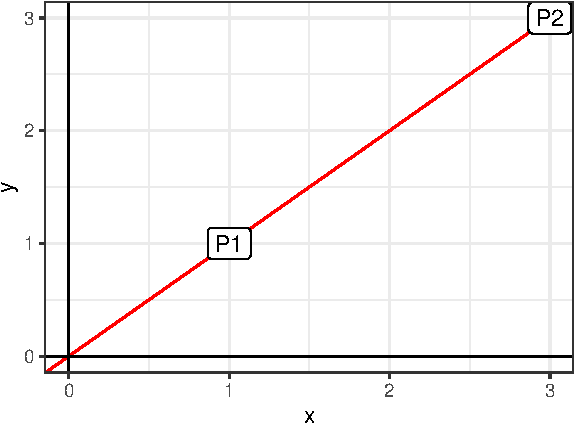
\includegraphics[width=0.28\linewidth]{production_economics_files/figure-beamer/linear-relationship-positive-1} \caption{Positive relationship between x and y variables}\label{fig:linear-relationship-positive1}
\end{figure}
\begin{figure}
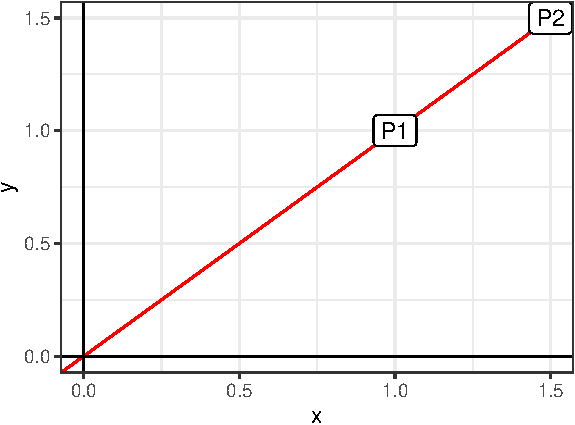
\includegraphics[width=0.28\linewidth]{production_economics_files/figure-beamer/linear-relationship-positive-2} \caption{Positive relationship between x and y variables}\label{fig:linear-relationship-positive2}
\end{figure}

\end{frame}

\begin{frame}{}
\protect\hypertarget{section-11}{}

\begin{figure}
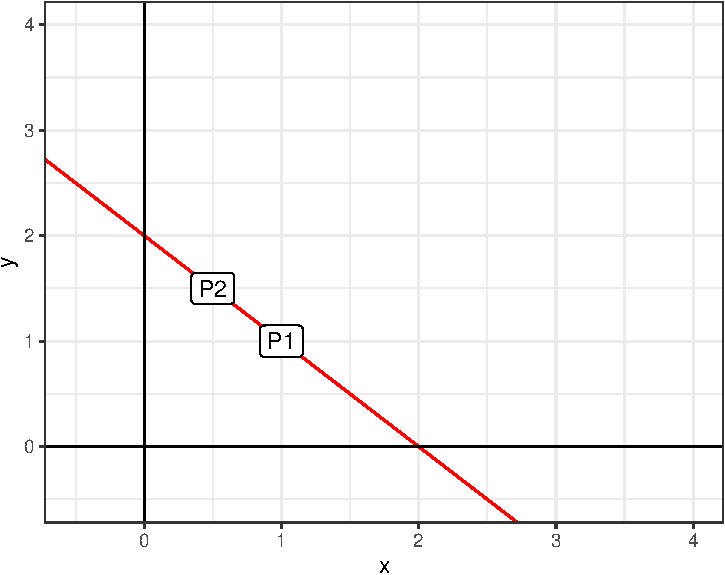
\includegraphics[width=0.45\linewidth]{production_economics_files/figure-beamer/linear-relationship-negative-1} \caption{Negative relationship between the two variables}\label{fig:linear-relationship-negative}
\end{figure}

The slopes of lines for first, second and third figures are,
respectively, +1, +1 and -1.

\end{frame}

\begin{frame}{}
\protect\hypertarget{section-12}{}

\[
Slope(P1P2) = \frac{P2_y - P1_y}{P2_x - P1_x}
\]

The slope of a line indicates the rate of change in one quantity in
response to the change in other; i.e., higher slopes (in magnitude)
correspond to faster changes in lower slopes (in magnitude) correspond
to slower changes.

\end{frame}

\begin{frame}{Non linear relationship graphs}
\protect\hypertarget{non-linear-relationship-graphs}{}

\begin{enumerate}
\tightlist
\item
  Monotonic
\end{enumerate}

\begin{itemize}
\tightlist
\item
  Monotonic functions are throughout either increasing or decreasing.
  Unlike the linear relationship, however, the rate or speed with which
  Y changes for a given change in X does not remain constant in all the
  ranges.
\item
  The rate of change at any point can be measured through drawing a
  tangent to the curve at that point.
\end{itemize}

\begin{enumerate}
\setcounter{enumi}{1}
\tightlist
\item
  Non-monotonic
\end{enumerate}

\begin{itemize}
\tightlist
\item
  In nonmonotonic functions, the nature of relationship itself changes
  through the range of the curve.
\end{itemize}

\end{frame}

\begin{frame}{Scatter diagram}
\protect\hypertarget{scatter-diagram}{}

\end{frame}

\begin{frame}{Slope of curve}
\protect\hypertarget{slope-of-curve}{}

\end{frame}

\hypertarget{product}{%
\section{Product}\label{product}}

\begin{frame}{Total product (TP)}
\protect\hypertarget{total-product-tp}{}

\begin{itemize}
\tightlist
\item
  A given level of total product is always associated with a particular
  level of input(s) use with a given technology. Production function is
  often presented as total output curve because total product curve and
  production function curve are closely associated.
\end{itemize}

\end{frame}

\begin{frame}{Average product (AP)}
\protect\hypertarget{average-product-ap}{}

\begin{itemize}
\tightlist
\item
  The term average product refers to the average productivity of
  resources. It is the ratio of total product (TP) to the quantity of
  input used in producing that amount of product, i.e., at any point on
  production function, it is the total output divided by the total input
  used.
\end{itemize}

\[
AP = \frac{Y}{X}
\]

Where Y is product and X the input(s).

\end{frame}

\begin{frame}{Marginal product}
\protect\hypertarget{marginal-product}{}

\begin{itemize}
\tightlist
\item
  The term marginal product refers to the quantity which additional
  (marginal) unit of factor-input adds to the total product. The
  marginal product (MP) at any level of the variable input can be
  approximated by dividing the addition to total output by the addition
  to total input:
\end{itemize}

\[
MP = \frac{\Delta Y}{\Delta X}
\]

Here, \(\Delta\) refers to the change in or addition to the product or
the input.

\begin{itemize}
\tightlist
\item
  It is the rate of change in total product at a given point as the
  quantity of input changes.
\item
  Although, average productivity provides some guidelines as to the
  manner in which resources are allocated, it is marginal productivity
  which provides the final criterion in determining optimum use of
  limited resources.
\end{itemize}

\end{frame}

\begin{frame}{Average marginal product}
\protect\hypertarget{average-marginal-product}{}

\begin{itemize}
\tightlist
\item
  The average marginal product indicates the productivity values between
  the two relevant input levels.
\end{itemize}

\begin{table}

\caption{\label{tab:marginal-product1}Example 1}
\centering
\fontsize{6}{8}\selectfont
\begin{tabular}[t]{rr}
\toprule
input & output\\
\midrule
0 & 10\\
5 & 20\\
10 & 30\\
15 & 40\\
\bottomrule
\end{tabular}
\end{table}

\begin{table}

\caption{\label{tab:marginal-product2}Example 2}
\centering
\fontsize{6}{8}\selectfont
\begin{tabular}[t]{rr}
\toprule
input & output\\
\midrule
0 & 10\\
5 & 30\\
10 & 45\\
15 & 50\\
\bottomrule
\end{tabular}
\end{table}

\end{frame}

\begin{frame}{}
\protect\hypertarget{section-13}{}

\begin{itemize}
\tightlist
\item
  In Example 1 (Table \ref{tab:marginal-product1}), when
  \(\Delta X = 5\), \(\Delta Y = 10\), then
  \(\frac{\Delta Y}{\Delta X} = \frac{10}{5} = 2.0\)
\item
  In Example 2 (Table \ref{tab:marginal-product2}), when
  \(\Delta X = 5\), \(\Delta Y = 20\) for first unit of input, 15 for
  second and 5 for third addition of input. It indicates that with each
  unit change in X from 0 to first addition of inputs, there is a change
  in 2 units of Y (\(\frac{\Delta Y}{\Delta X} = \frac{20}{5} = 4.0\)).
  The Marginal product of variable unit can be thus approximated by
  dividing addition to total output by addition to total input. The
  marginal product, however, has decreased upon further addition of
  inputs to the first input level. i.e., when the input level is 15 (0 +
  5 + 10), the additional 5 (10-5) unit input have given rise to only 15
  (45-30) unit of output, hence the marginal product
  (\(\frac{\Delta Y}{\Delta X} = \frac{15}{5} = 3.0\)). This is
  reduction from the previous value of MP of 4.
\end{itemize}

\end{frame}

\begin{frame}{Exact marginal product}
\protect\hypertarget{exact-marginal-product}{}

\begin{itemize}
\item
  Exact (point) marginal product refers to the marginal product as a
  derivative. This indicates the marginal product of a point. The
  derivative gives the values at a point and not an average between two
  points.
\item
  If the production function \(Y = \alpha + \beta X\), point marginal
  product = \(\frac{\delta Y}{\delta X} = b\), which is a linear
  constant relationship. If the production function is non-linear, i.e.,
  \(Y = \alpha + \beta X + \gamma X^2\), exact MP will be
  \(\frac{\delta Y}{\delta X} = \beta + 2\gamma X\).
\end{itemize}

\end{frame}

\begin{frame}{Marginal cost}
\protect\hypertarget{marginal-cost}{}

\begin{itemize}
\tightlist
\item
  The additional cost of doing a little bit more (or 1 unit more if a
  unit can be measured) of an activity.
\item
  How do you make a rational decision about when the alarm should go
  off? What you have to do is to weigh up the costs and benefits of
  additional sleep. Each extra minute in bed gives you more sleep (the
  marginal benefit), but gives you more of a rush when you get up (the
  marginal cost).
\item
  The decision is therefore based on the costs and benefits of extra
  sleep, not on the total costs and benefits of a whole night's sleep.
\end{itemize}

\begin{block}{Rational decision}

\begin{itemize}
\tightlist
\item
  Doing more of an activity if its marginal benefit exceeds its marginal
  cost and doing less if its marginal cost exceeds its marginal benefit.
\item
  Rational decisions are made with rational choices; that involve
  weighing up the benefit of any activity against its opportunity cost.
\end{itemize}

\end{block}

\end{frame}

\hypertarget{bibliography}{%
\section{Bibliography}\label{bibliography}}

\begin{frame}{For more information}
\protect\hypertarget{for-more-information}{}

\end{frame}




\end{document}
